% Proposal (3.5p)
\label{sec:proposal}


% Gena: Are you really following this approach???
%The rationale behind our approach is the following: an external agent (user or another system) creates a \emph{deployment request}, with goals that should be achieved in a given computing environment. A deployment agent, is responsible to handle that \emph{deployment request} autonomously. The deployment agent is capable of discover available resources in a computing environment it manages. That knowledge about the computing environment is the \emph{context} for the target deployment. The deployment agent is also capable of choosing artifacts from a repository that allows the satisfaction of the deployment request. The process of choosing the correct set of artifacts to allow the deployment request satisfaction is the \emph{deployment planning}.

% General discussion
Following the model proposed by Andersson et al.\cite{andersson_software_2013} for adaptive software development process, we divide our approach into \emph{offline} and \emph{online} activities. In this work, the \emph{offline} activities are conducted by software engineers, and result in development and publishing of software components. The \emph{online} activities are autonomously executed in target environment, and result in the deployment of the system. Figure~\ref{fig:overview} presents an overview of the process.

\begin{figure*}[!htb]
  \centering
  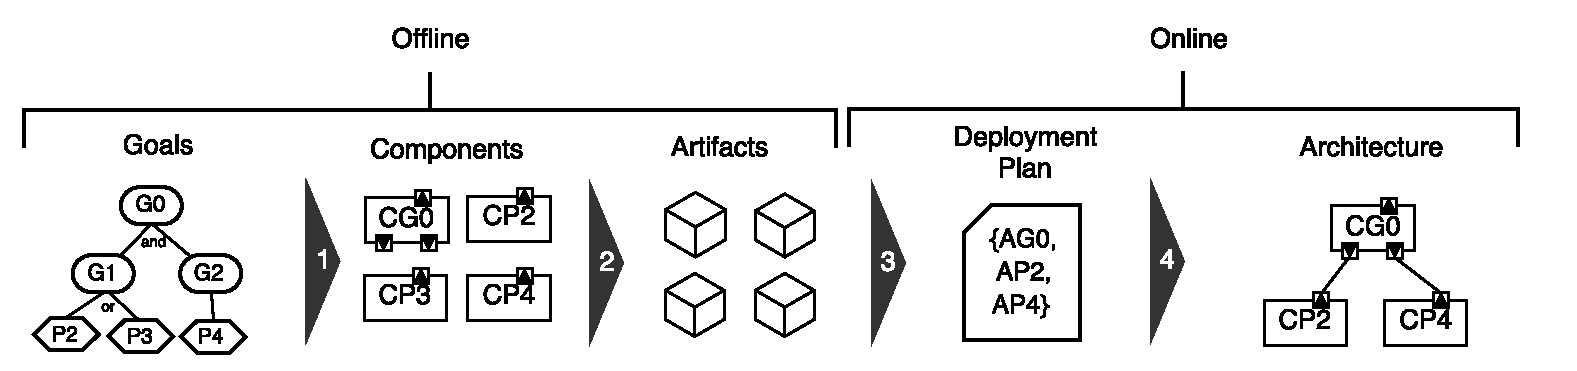
\includegraphics[width=1\linewidth]{transformations}
  \caption{Activities: (1) component mapping; (2) packaging; (3) deployment planning; (4) component binding}
\label{fig:overview}
\end{figure*}


In the offline part, occurs the design of the application. In the first step of our approach, components are mapped from the system CGM using patterns. In the second, these components are packaged into artifacts together with their metadata, which describes what goals the artifact provides, its context conditions and dependencies. These packaged artifacts are put in a repository.

In the online part of the approach, the Goalp deployment planning is executed in the target computing environment and autonomously finds a deployment plan.
The deployment planning is responsible to look into the repository of artifacts and based on context information and goals, find a set of artifacts that should be deployed to the target computing environment in order to make the goals achievable.

\section{From Goals To Artifacts}

Previously, goal-driven  approaches were proposed for introducing variability at requirements, context modeling, software behavior, and software architecture\cite{angelopoulos_capturing_2015}\cite{yu_goals_2008}.
In our methodology, we propose a systematic approach to support deployment variability, from requirements to deployment.
Deployment variability is important since not taking into account the heterogeneity of a computing environment may lead to unnecessary or even unsuited deployment of components.
Such scenario would bring a negative impact to software performance, or in some cases represent inconsistent deployment of functionalities on the target device.


When developing a monolithic software, we implement in the same codebase all functionalities, then all code is built and deployed together.
In the Filling Station Advisor example, if implementing it as a monolic software, the logic to get the vehicle position using GPS or antenna triangulation would stay in the same codebase and would be deployed altogether in the target environment, even when it does not have antenna triangulation capability.

% Interfaces create architecture independency. Yet, even using interfaces we can can have static dependencies at some point, at the implementation instantiation. Using reflexive platforms we eliminate the static dependency as the platform can find available interfaces implementations at runtime.
% To create deployment independency we can use interfaces and polymorphic resources of software platforms.

% To achieve a root goal we need to get position.
% We create an interface that describe that service.
% We create implementations of that interface as components.
% That components are packaged in different artifacts. We have static dependency of the component with the interface that it implements.
% Also we have a static dependency between an a component and the interfaces that describes the services it depends on.
% The interfaces and its dependencies (it being clients or implementations) can be packaged separately.
% We have an implementation dependency between a client components and any component that implements the service it depends on. That dependency can be resolved late on, in deployment time.

In order to better cope with heterogeneity in the computing environment we should minimize the coupling between parts of the code that have dependencies of specific resources in the environment.
By encapsulating dependencies of specific resources into components, it is possible to create variability at architecture level. By packaging the components into different artifacts, it is possible to maintain such variability at deployment level. Such variability is useful as it allows the deployment of components only to environment that have the required resources.

Regarding the Filling Station Advisor example, depicted in \ref{fig:goal_model_filling_station_advisor}, for goal \emph{G1}(Get Position), components can be implemented providing the actual position of the device by means of GPS or antenna triangulation. These components can be packaged into different artifacts that will only be deployed when the target environment has the appropriate resources.

\subsection{CGM for heterogeneous computing environments}
\label{context}

A systematic way of analysing the capabilities of the computing environment is needed in order to support the resolution of variability at deployment-time. First, the available capabilities in the environment should be represented in the context.

\begin{defn}[Resource]

  A resource provides a specific computing capability, it could be available in the computing environment and used in plans. A resources receives a label.

\end{defn}

Regarding the Filling Station Advisor, relevant resources are \emph{GPS}, \emph{Antenna Triangulation}, \emph{Internet connection}, \emph{storage}, etc.

\begin{defn}[Context]

  A context Ctx := r1..rn, \{ r $\in$ Ctx | a resource labeled r is available in the computing environment\}
\end{defn}

Context is a set of labels. In our example, the set [gps-capability,
internet-connection, synthesized-voice] is a an example of context, representing that GPS, connection to the Internet and voice synthesizing are resources available in the computing environment.

Then, the applicability of a plan should be related with available resources. Conditions represent restrictions related with the environment, and can be evaluated against the context.

\begin{defn}[Context condition]
  A context condition cx:=TRUE iff cx:r, r $\in$ Ctx
\end{defn}

A context condition is satisfied if the associated resource is present in the context.
In a scenario with context Ctx=[gps, internet-connection], the context condition c1:gps holds.

As proposed by Rain at al~\cite{ali_goal-based_2010}, context conditions are used to solve variability. In Figure~\ref{fig:goal_model_filling_station_advisor}, the goal G1 has two alternatives to be achieved: by executing plan P1 or P2. The plan P1 is applicable if the context condition c1 holds, which is the case when GPS is available in the environment.


\subsection{Preparing Components}

\subsubsection{Goals to Components}
\label{sec:goals_components}
Components are architectural units. In our proposal, components definitions are mapped from the CGM and them developed by the architect/developer.

The patterns present in table~\ref{table_cgm_to_components_patterns} are used to map components based on the CGM of the system. By mapping components we mean identifying which component should be developed in order to reflect the CGM of the system. By using the proposed patterns, the variability present in the CGM is kept at architecture of the system. Theses patterns are an extension of Yu et al.\cite{yu_goals_2008} patterns for the Goals-Component view, with contextual conditions.

\begin{table}[!]
\centering
\caption{Contextual Goal Model to components; (1) And-refinement, (2)OR-refinement, (1) context condition, }
\label{table_cgm_to_components_patterns}
\bigskip
\begin{tabular}{|c p{5cm}|}
\hline
 %\textbf{ A } & \textbf{ B} & \textbf{C} \\ \hline
 \raisebox{-\totalheight}{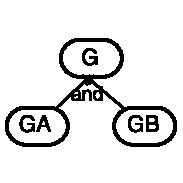
\includegraphics[scale=.7]{patterns_and}} &
 \begin{lstlisting}
 Component CG {
   provides IG;
   requires
      IGA, IGB;
 }
 \end{lstlisting} \\ \hline
 \raisebox{-\totalheight}{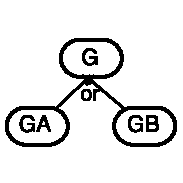
\includegraphics[scale=.7]{patterns_or}} &
 \begin{lstlisting}
 Component CG {
   provides IGA;
 }
 Component CG {
   provides IGB;
 }
 \end{lstlisting} \\ \hline
 \raisebox{-\totalheight}{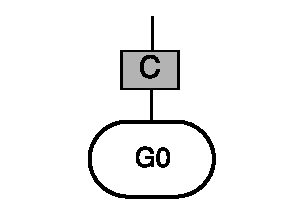
\includegraphics[scale=.7]{patterns_condition}} &
 \begin{lstlisting}
 Component CG {
   provides IG;
   condition C;
 }
 \end{lstlisting} \\ \hline
\end{tabular}
\end{table}
The presented patterns are described using goals, but they can be applied for goals and plans, without distinction.

And-refinement result in components that define a strategy to achieve a given goal by achieving two or more sub more concrete goals.
Mapping components from a Goal And-refinemnt result in: (i) a root interface that describe what component provides. (ii) Interfaces for each sub goal. (iii) A component that provides the interface (i) and requires each interface generated for sub goals (ii). That component (iii), implements a strategy to achieve its provided goal. It coordinates the sub more specific goals by calling then, and passing one result as input on another, when applicable.
As an example, applying And-refinement patterns for Root Goal G0 of the Filling Station Advisor application, will result in interface IG0 and a component G0 that provides IG0 and requires IG1, IG2, IG3, IG4, and IG5.
\begin{lstlisting}
  Component G0 {
    provides IG0;
    requires IG1, IG2, IG3, IG4,IG5;
  }
\end{lstlisting}

Applying or-refinements pattern, results in a root interface definition and in multiple implementation. When Or-refinements is associated with context-conditions, it allows for alternative strategies using different resources in the computing environment. For example, in the Filling Station Advisor, applying the patterns for G1, P1 and P2 will result in the following components:

\begin{lstlisting}
  Component CP1 {
    provides IG1;
    condition C1;
  }
  Component CP2 {
    provides IG1;
    condition C2;
  }
\end{lstlisting}

The two plans P1 and P2 associated with the Or-refinement has different context conditions (C1:gps and C2:antenna triangulation).
That variability in the design allows for the adaptation to the heterogeneity in the target environment.

\subsubsection{Artifacts}
\label{sec_artifacts}

From the deployment point of view, the components and interfaces should be packaged in an file archive to distribution. We name such file an artifact.
An artifact should follow a standard packaging schema, so it can be manipulated by a package manager.
In our approach, we propose to include into the artifact metadata that describe the artifact provided goals, context conditions, and dependencies. That metadata reflect information about the packaged components. For our approach, the metadata of interest is the following:

\begin{description}
  \item[Provided goals:] goals that can be made achievable by successfully deploying the component.
  \item[Context conditions:] conditions that can be evaluated against the context. If the conditions are not satisfied it means that the component can not be deployed at the given context. This is the case when the artifact required resources are not available in the computing environment.
  \item[Dependencies:] required goals that should be provided by other artifacts.
\end{description}

When creating the artifact we can calculate the metadata by looking at the packaged components. The artifact \emph{provided goals} metadata are the union of all \emph{provided goals} of the components packaged in this artifact. The same is valid for \emph{context conditions} and \emph{dependencies} metadata.

Both \emph{context conditions} and \emph{dependencies} impose restrictions on when an artifact can be deployed.
Context conditions refer to the need on resources in the computing environment that are beyond the deployment agent capacity of management. Such dependency can be related to hardware implementation, e.g. GPS-module, our platform lower level software implementation and access authorization, e.g. access to vehicle on-board computer data. If a context condition do not hold there is nothing that can be done at deployment time to change that.
Dependencies, differently, refer to the need on another artifacts. It is specified in the terms of Provided Goals. Like another dependency management approaches, an artifact can depends on another artifacts.
Different from other approaches, we specify the dependency not to a specific version of an artifact identification but in terms of what an artifact provides.
So, in the Filling Station Advisor, the artifact A0, that packs the component G0 depends on IG0-definition and IG0. To satisfy the dependency an artifacts that provides IG0-definition should be available, as well as at least one artifact that implements IG0.

Artifacts are registered in a repository which allows the distribution of artifacts to target environment. In the registration process, the artifact is upload to the repository, its metadata is read, and registered in the repository database.

\subsubsection{Deployment Architectural Style}
\label{depl_arch_style}

In order to maximize the flexibility of systems implemented using Goalp deployment approach, is proposed an architectural style for creating artifacts.

Artifacts can have be of 3 types:

\begin{description}
  \item[Definition] artifacts that specify the interface of goals. It contains interfaces declarations and data model. It specify the API or contracts for a given set of goals.
  The advantage of separating the goals declaration in a specific artifact is creating implementation independence.
  Goals declarations depends only on other goals declarations and have no context conditions. Goals declarations do not provide any goals.

  \item[Strategy] artifacts that package components that result from AND-refinements. A Goal refinement provides a high level goal and depends on other more refined goals. It should have no context condition as it do not implement plans that use specific resources in the computing environment.

  \item[Plan implementation] theses artifacts contain the domain logic implementation. The plan could have dependencies on specific resources on the computing environment. In a dependency tree we have plan implementation artifacts as leafs.
  Plan implementation artifacts provides low-level goals and can have dependencies and context conditions.

\end{description}

These types of components has not different treatment by the deployment planning but following it will increase the flexibility of deployment.


\section{The Process}

\subsubsection{Roles}
The proposed process considers three roles: users, requirements engineers and software architects.
Figure~\ref{fig:process_roles} summarize the collaboration between the roles.

 \begin{figure}[!htb]
   \centering
   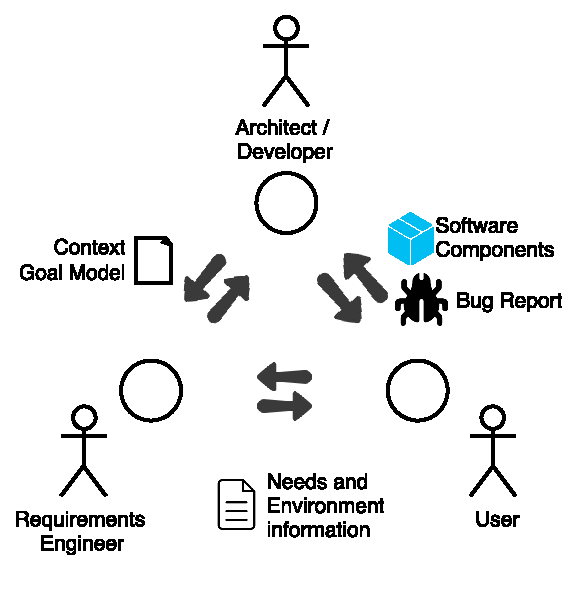
\includegraphics[width=.4\linewidth]{process_roles}
   \caption{Roles collaboration}
 \label{fig:process_roles}
 \end{figure}

\begin{description}
  \item[User]
  This role has access to a particular computing environment and want to achieve some goals there.
  \item[Requirements Engineer]
  Is responsible to translate users goals to a contextual goal model. Also is responsible to analyze the different contexts that the system is meant to operate and how it affects the goals.
  \item[Architect] Architect project the software architecture such as to permit variability of deployment.
  From the point of view of dynamic heterogeneous computing environments, the focus is to create interfaces for components that can allow for goal achievements using different computing resources.

\end{description}



\subsubsection{Activities}

Figure~\ref{fig:deployment_process_flow} describe the development process activities.

\label{sub:Proposal}
\begin{figure}[!htb]
  \centering
  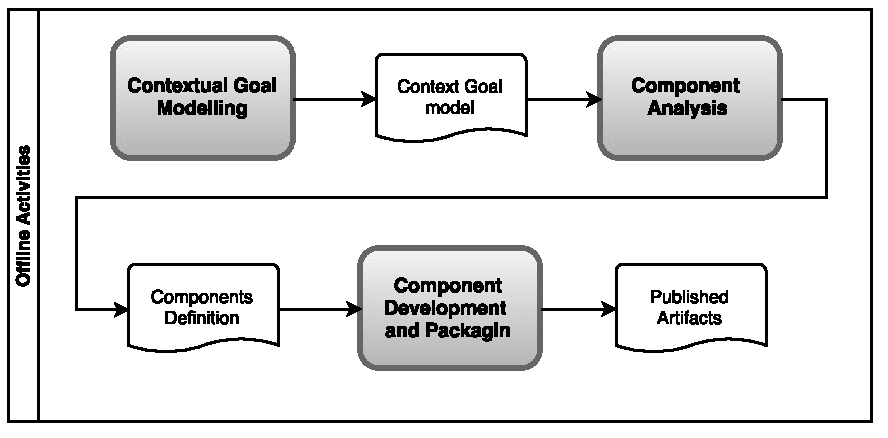
\includegraphics[width=\linewidth]{deployment_process_flow}
  \caption{Deployment Process Activities}
\label{fig:deployment_process_flow}
\end{figure}

\subsubsection{Goal Modeling}
This phase is coordinated by a requirement engineer with participation of a domain specialist, possibly the user.
A process such as TROPOS can be used. The output of this phase is a goal model.
Here, the goal model assumes a central role in the software development process. The goal model besides define the space of the solution, also works as common language. The goal model formalize the domain knowledge. It defines a common language between user and developers that will allow software deployment driven by user goals.


\subsubsection{Context Goal Modeling}
In this phase, the Goal model should be annotated with \emph{context conditions} related with the computing environment. That analysis is a context analysis and could benefit of the process described in~\cite{ali_goal-based_2010}. The requirements engineer should use knowledge about the computing resources that may be available at the computing environment.


\subsubsection{Component Analysis}
Software engineer should identify variability points.
Variability points in the contextual goal model are points where goals can be achieve with different strategies, each one having different context conditions.
Component interfaces are created following the guidelines described in Section~\ref{sec:goals_components}. The input and output of components are defined.

Also at this phase, it should be defined the sensors needed to evaluate facts about the computing environment.

\subsubsection{Component Development and Packaging}

Component development includes the cycle coding, build and test of software components.
The component package in the standard packaging schema is an artifact and should be put in a delivery system.
